\documentclass{article}

\usepackage{kotex}
\usepackage{amssymb}
\usepackage{graphicx}

\graphicspath{ {./images/} }

\renewcommand{\figurename}{그림}
\renewcommand{\tablename}{표}

\title{Mirésatanä 2 데이터시트}
\author{아이즌 Z. 스치 @ Lofanfashasch 1013193}

\begin{document}

\maketitle
\tableofcontents

\pagebreak

\section{개요}

Mirésatanä 2는 로지심에서 작동하는 8비트 컴퓨터를 만들기 위한 프로젝트이다.
이전 버전인 mycomputer에서 일반 길이의 데이터 주소를 구현하기 위해 시작되었으며,
8비트 주소를 사용하는 것을 목표로 하고있다.

Mirésatanä는 현존하는 여러 컴퓨터의 기능들에서 영감을 받아
직관적으로 제작되고 있으며, 실제 컴퓨터 내부 구조를 이루는 부품들과
기능·구조상의 차이가 있을 수 있다.

mycomputer의 개발은 2023년 3월에 진행되었으며,
Mirésatanä의 개발은 2023년 4월에 시작되었다.

\section{부품 설계}

\subsection{ArithmeticLogicBit}

ArithmeticLogicBit는 논리곱과 배타적 논리합,
전가산 결과를 출력하는 ArithmeticLogic의 구성 부품이다.

ArithmeticLogicBit는
$A$, $B$, $C_i$, $N$, $X$의 입력 핀과
$C_o$, $O$의 출력 핀을 가지고 있고,
각각은 다음을 의미한다.

\begin{itemize}
    \item $A$ -- A. 연산의 첫 번째 인자가 될 비트
    \item $B$ -- B. 연산의 두 번째 인자가 될 비트
    \item $C_i$ -- Carry In. 이전 가산기에서 발생한 올림 비트
    \item $N$ -- aNd enable. $O$가 $A \veebar B$를 출력하게 만드는 비트
    \item $X$ -- Xor enable. $O$가 $AB$를 출력하게 만드는 비트
    \item $C_o$ -- Carry Out. 가산 연산 중 발생한 올림 비트
    \item $O$ -- Output. 연산의 결과
\end{itemize}

ArithmeticLogicBit의 진리표는 \tablename{} \ref{tab:alb}과 같이 주어진다.

\begin{table}[h]
    \centering
    \begin{tabular}{ccccc|cc}
        $A$ & $B$ & $C_i$ & $N$ & $X$ & $C_o$ & $O$ \\
        \hline
        $A$ & $B$ & $C_i$ &  0 &  0 & $AB + BC_i + C_iA$ & $A \oplus B \oplus C_i$ \\
        $A$ & $B$ & $C_i$ &  0 &  1 &  0 & $A \oplus B$ \\
        $A$ & $B$ & $C_i$ &  1 &  0 &  0 & $AB$ \\
    \end{tabular}
    \caption{ArithmeticLogicBit의 진리표}
    \label{tab:alb}
\end{table}

\figurename{} \ref{fig:alb}은 ArithmeticLogicBit의 회로도이다.

\begin{figure}[h]
    \centering
    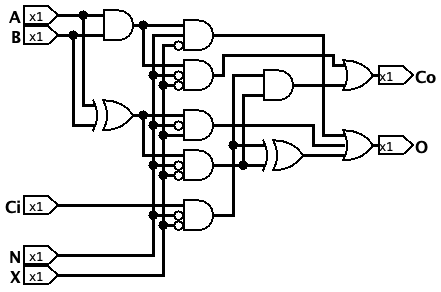
\includegraphics[scale=0.5]{ArithmeticLogicBit} \\
    \caption{ArithmeticLogicBit의 회로도}
    \label{fig:alb}
\end{figure}

\subsection{ArithmeticLogic}

ArithmeticLogic은 8비트 정수의 산술 연산과 논리 연산을 수행하는 부품이다.

ArithmeticLogic은 $A$, $B$, $I_A$, $I_B$, $I_O$, $B_e$, $N$, $X$, $C_i$의 입력 핀과
$O$, $C_o$의 출력 핀을 가지고 있다.
이중에서 $A$, $B$, $O$는 8비트 핀이다.
각각은 다음을 의미한다.

\begin{itemize}
    \item $A$ -- A. 연산의 첫 번째 인자가 될 수
    \item $B$ -- B. 연산의 두 번째 인자가 될 수
    \item $I_A$ -- Invert A. $A$의 결과를 반전하여 연산을 진행한다.
    \item $I_B$ -- Invert B. $\neg B$를 내부 두 번째 인자 입력에 논리합한다.
    \item $I_O$ -- Invert O. $O$의 결과를 반전하여 출력한다.
    \item $B_e$ -- B Enable. $B$를 내부 두 번째 인자 입력에 논리합한다.
    \item $N$ -- aNd enable. 두 수의 논리곱을 $O$에 출력한다.
    \item $X$ -- Xor enable. 두 수의 배타적 논리합을 $O$에 출력한다.
    \item $C_i$ -- Carry In. 가산 연산에 반영할 올림 비트
    \item $O$ -- Output. 연산의 결과
    \item $C_o$ -- Carry Out. 가산 연산에서 발생한 올림 비트
\end{itemize}

ArithmeticLogic은 입력되는 옵션에 따라 두 인자 $A$, $B$에 대한
$A$, $\neg A$, $A+1$, $A-1$, $A+B$, $A-B$, $-A$, $B-A$,
$A \veebar B$, $\neg(A \veebar B)$, $A\wedge B$, $\neg (A \wedge B)$, $A \vee B$, $\neg(A \vee B)$ 등을
계산할 수 있다.

ArithmeticLogic은 \tablename{} \ref{tab:al}와 같은 진리표를 가진다.
논리합($\vee$)과 산술합($+$) 연산에 주의해야 한다.

\begin{table}[p]
    \centering
    \begin{tabular}{cc|ccccccc|ll}
        $A$ & $B$ & $I_A$ & $I_B$ & $I_O$ & $B_e$ & $N$ & $X$ & $C_i$ & $O$ & $C_i$ \\
        \hline
        $A$ & $B$ & 0 & 0 & 0 & 0 & - & - & 0 & $A$ & 0 \\
        $A$ & $B$ & 0 & 0 & 0 & 0 & - & - & 1 & $A + 1$ & $\forall A$ \\
        $A$ & $B$ & 0 & 0 & 0 & 1 & 0 & 0 & 0 & $A + B$ & - \\
        $A$ & $B$ & 0 & 0 & 0 & 1 & 0 & 0 & 1 & $A + B + 1$ & - \\
        $A$ & $B$ & 0 & 0 & 0 & 1 & 0 & 1 & 0 & $A \veebar B$ & 0 \\
        $A$ & $B$ & 0 & 0 & 0 & 1 & 1 & 0 & 0 & $A \wedge B$ & 0 \\
        $A$ & $B$ & 0 & 0 & 1 & 0 & - & - & 0 & $\neg A$ & 0 \\
        $A$ & $B$ & 0 & 0 & 1 & 1 & 0 & 1 & 0 & $\neg(A \veebar B)$ & 0 \\
        $A$ & $B$ & 0 & 0 & 1 & 1 & 1 & 0 & 0 & $\neg(A \wedge B)$ & 0 \\
        $A$ & $B$ & 0 & 1 & 0 & 0 & 0 & 0 & 0 & $A - B - 1$ & $A > B$\\
        $A$ & $B$ & 0 & 1 & 0 & 0 & 0 & 0 & 1 & $A - B$ & $A \geq B$\\
        $A$ & $B$ & 0 & 1 & 0 & 1 & 0 & 0 & 0 & $A - 1$ & $\exists A$\\
        $A$ & $B$ & 0 & 1 & 1 & 0 & 0 & 0 & 0 & $B - A$ & $A > B$\\
        $A$ & $B$ & 0 & 1 & 1 & 0 & 0 & 0 & 1 & $B - A - 1$ & $A \geq B$\\
        $A$ & $B$ & 1 & 0 & 0 & 0 & 0 & 0 & 0 & $\neg A$ & 0 \\
        $A$ & $B$ & 1 & 0 & 0 & 0 & 0 & 0 & 1 & $-A$ & $\forall A$ \\
        $A$ & $B$ & 1 & 0 & 0 & 1 & 0 & 0 & 0 & $B - A - 1$ & - \\
        $A$ & $B$ & 1 & 0 & 0 & 1 & 0 & 0 & 1 & $B - A$ & - \\
        $A$ & $B$ & 1 & 1 & 0 & 0 & 0 & 0 & 0 & $-A-B-2$ & - \\
        $A$ & $B$ & 1 & 1 & 0 & 0 & 0 & 0 & 1 & $-A-B-1$ & - \\
        $A$ & $B$ & 1 & 1 & 0 & 0 & 1 & 0 & 0 & $\neg(A \vee B)$ & - \\
        $A$ & $B$ & 1 & 1 & 0 & 1 & 0 & 0 & 0 & $-A-2$ & $\neg \forall A$ \\
        $A$ & $B$ & 1 & 1 & 0 & 1 & 0 & 0 & 1 & $-A-1$ & 1 \\
        $A$ & $B$ & 1 & 1 & 1 & 0 & 1 & 0 & 0 & $A \vee B$ & 0 \\
    \end{tabular}
    \caption{ArithmeticLogic}
    \label{tab:al}
\end{table}

\figurename{} \ref{fig:al}은 ArithmeticLogic의 회로도이다.

\begin{figure}[p]
    \centering
    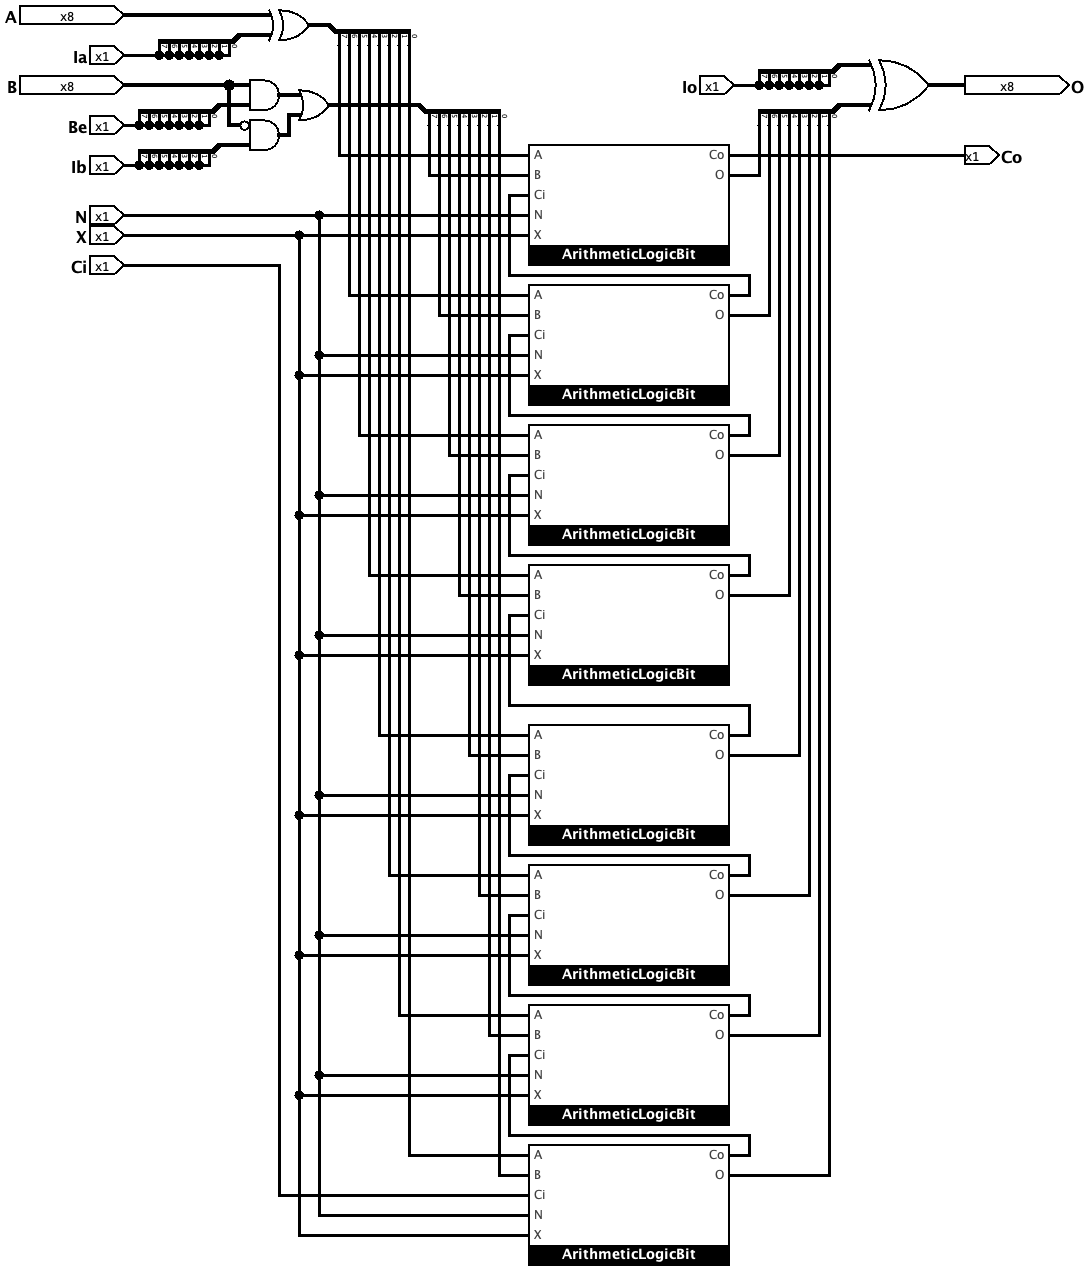
\includegraphics[scale=0.35]{ArithmeticLogic} \\
    \caption{ArithmeticLogic의 회로도}
    \label{fig:al}
\end{figure}

\pagebreak

\subsection{Shiftre}

Shiftre는 입력된 값에 대한 1회 좌측·우측 시프트 연산 결과를 출력하는
부품이다.

Shiftre는 $I$, $S$, $R$, $L$의 입력 핀과
$O$, $O_l$, $O_r$의 출력 핀을 가지고 있다.
이중에서 $I$, $O$는 8비트 핀이다.
각각은 다음을 의미한다.

\begin{itemize}
    \item $I$ -- Input. 시프트 연산을 수행할 정수
    \item $E$ -- Enable. 시프트 연산 수행의 여부.
        0으로 설정된 경우에는 연산을 수행하지 않고,
        1로 설정된 경우에는 연산을 수행한다.
    \item $R$ -- Right. 시프트 방향을 오른쪽으로 설정한다.
        0으로 설정된 경우에는 왼쪽 시프트를 수행한다.
    \item $L$ -- Logical. 오른쪽 시프트를 수행하는 경우에,
        논리적 시프트와 산술적 시프트 중에서 선택한다.
        0으로 설정된 경우에는 산술적 시프트를 수행하고,
        1로 설정된 경우에는 논리적 시프트를 수행한다.
    \item $O$ -- Output. 시프트 결과
    \item $O_l$ -- Overflow Left. 왼쪽 시프트 수행 중에 오버플로우가 발생함
    \item $O_r$ -- Overflow Right. 오른쪽 시프트 수행 중에 오버플로우가 발생함
\end{itemize}

\tablename{} \ref{tab:shr}은 Shiftre의 표이다.

\begin{table}[h]
    \centering
    \begin{tabular}{c|ccc|ccc}
        $I$ & $E$ & $R$ & $L$ & $O$ & $O_l$ & $O_r$ \\
        \hline
        \texttt{abcd efgh} & 0 & - & - & \texttt{abcd efgh} & 0 & 0 \\
        \texttt{abcd efgh} & 1 & 0 & - & \texttt{bcde fgh0} & \texttt a & 0 \\
        \texttt{abcd efgh} & 1 & 1 & 0 & \texttt{aabc defg} & 0 & \texttt h \\
        \texttt{abcd efgh} & 1 & 1 & 1 & \texttt{0abc defg} & 0 & \texttt h \\
    \end{tabular}
    \caption{Shiftre의 진리표}
    \label{tab:shr}
\end{table}

\figurename{} \ref{fig:shr}은 Shiftre의 회로도이다.

\begin{figure}[p]
    \centering
    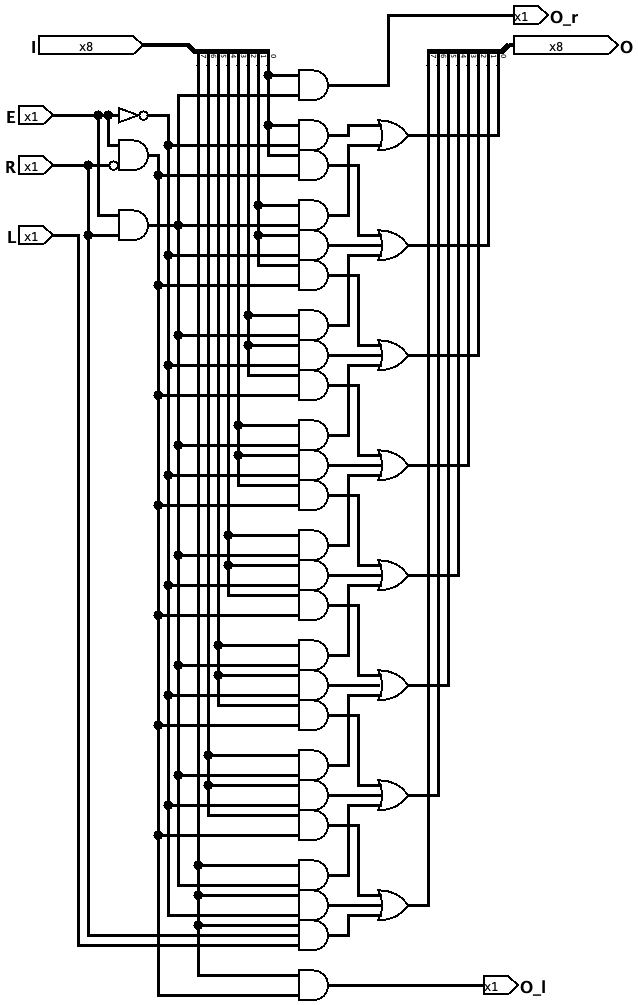
\includegraphics[scale=0.5]{Shiftre} \\
    \caption{Shiftre의 회로도}
    \label{fig:shr}
\end{figure}

\pagebreak

\subsection{OpCodeToFlags}

OpCodeToFlags는 4비트 연산자 코드를 ArithmeticLogic 플래그로 변환해주는
부품이다.

OpCodeToFlags는 $O_c$의 입력 핀과
$I_A$, $I_B$, $I_O$, $B_e$, $N$, $X$, $C_i$, $E$, $R$, $L$ 출력 핀을 가지고 있다.
이중에서 $O_c$는 4비트 입력 핀이다.
$I_A$, $I_B$, $I_O$, $B_e$, $N$, $X$, $C_i$는 ArithmeticLogic에 입력되는 핀이고
$E$, $R$, $L$는 Shiftre에 입력되는 핀이다.

OpCodeToFlags의 진리표는 \tablename{} \ref{tab:octf}과 같다.
기울인꼴로 표현된 것은 무관조건이다.

\begin{table}[h]
    \centering
    \begin{tabular}{cl||ccccccc|ccc}
        $O_c$ & 연산자 & $I_A$ & $I_B$ & $I_O$ & $B_e$ & $N$ & $X$ & $C_i$ & $E$ & $R$ & $L$ \\
        \hline
        \texttt{0} & A    & 0 & 0 & 0 & 0 & \textit 0 & \textit 1 & 0 & 0 & \textit 0 & \textit 0 \\
        \texttt{1} & NOT  & 1 & 0 & 0 & 0 & \textit 0 & \textit 1 & 0 & 0 & \textit 0 & \textit 1 \\
        \texttt{2} & NEG  & 1 & 0 & 0 & 0 & \textit 1 & \textit 0 & 1 & 0 & \textit 0 & \textit 0 \\
        \texttt{3} & SHL  & 0 & 0 & 0 & 0 & \textit 1 & \textit 0 & 0 & 1 & 0 & \textit 1\\
        \texttt{4} & INC  & 0 & 0 & 0 & 0 & \textit 0 & \textit 0 & 1 & 0 & \textit 1& \textit 0 \\
        \texttt{5} & DEC  & 0 & 1 & 0 & 1 & 0 & 0 & 0 & 0 & \textit 1& \textit 1\\
        \texttt{6} & ADD  & 0 & 0 & 0 & 1 & 0 & 0 & 0 & 0 & \textit 1& \textit 0 \\
        \texttt{7} & SUB  & 0 & 1 & 0 & 0 & 0 & 0 & 1 & 0 & \textit 1& \textit 1\\
        \texttt{8} & XOR  & 0 & 0 & 0 & 1 & 0 & 1 & 0 & 0 & \textit 0 & \textit 0 \\
        \texttt{9} & XNOR & 0 & 0 & 1 & 1 & 0 & 1 & 0 & 0 & \textit 0 & \textit 1\\
        \texttt{A} & AND  & 0 & 0 & 0 & 1 & 1 & 0 & 0 & 0 & \textit 0 & \textit 0 \\
        \texttt{B} & NAND & 0 & 0 & 1 & 1 & 1 & 0 & 0 & 0 & \textit 0 & \textit 1\\
        \texttt{C} & OR   & 1 & 1 & 1 & 0 & 1 & 0 & 0 & 0 & \textit 1& \textit 0 \\
        \texttt{D} & NOR  & 1 & 1 & 0 & 0 & 1 & 0 & 0 & 0 & \textit 1& \textit 1\\
        \texttt{E} & ASR  & 0 & 0 & 0 & 0 & \textit 1& \textit 0 & 0 & 1 & 1 & 0 \\
        \texttt{F} & LSR  & 0 & 0 & 0 & 0 & \textit 1& \textit 0 & 0 & 1 & 1 & 1 \\
    \end{tabular}
    \caption{OpCodeToFlags의 진리표}
    \label{tab:octf}
\end{table}

OpCodeToFlags의 회로도는 \figurename{} \ref{fig:octf}과 같다.

\begin{figure}[p]
    \centering
    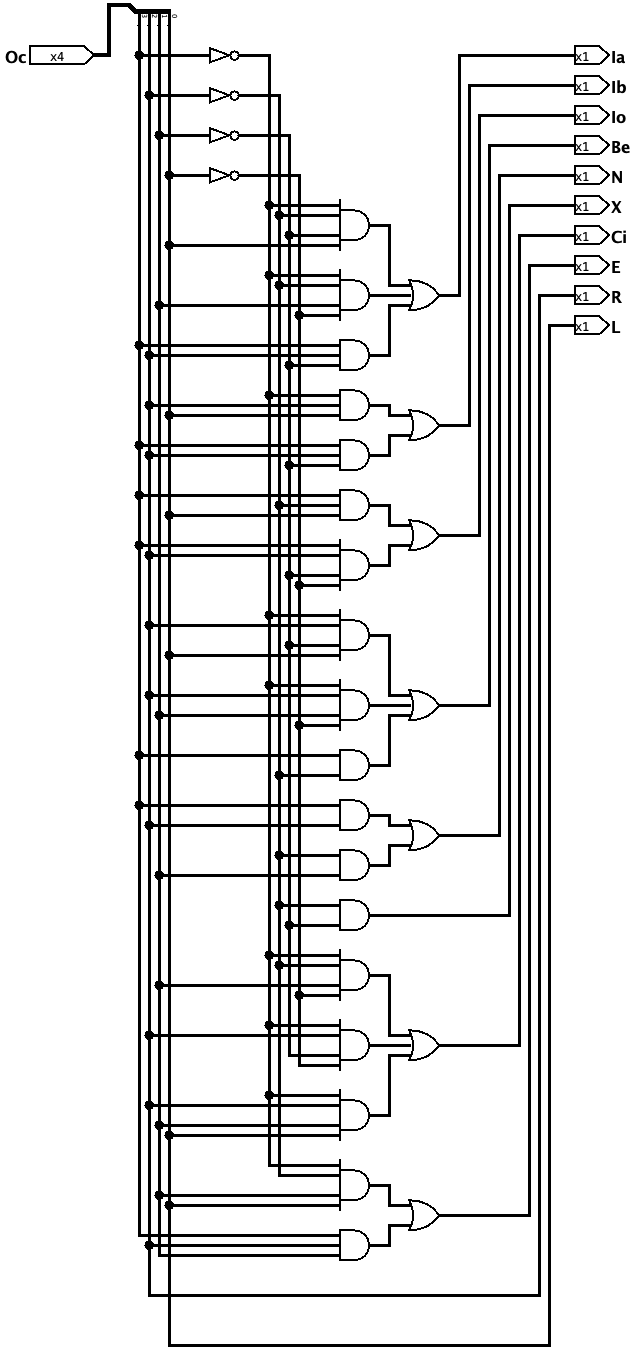
\includegraphics[scale=0.35]{OpCodeToFlags} \\
    \caption{OpCodeToFlags의 회로도}
    \label{fig:octf}
\end{figure}

\pagebreak

\subsection{ALU}

ALU는 Arithmetic Logical Unit의 약자로,
산술 연산과 논리 연산을 수행하고 그 결과를 출력하는 부품이다.

ALU는 $A$, $B$, $O_c$의 입력 핀과
$O$, $F_v$, $F_c$, $F_s$, $F_z$의 출력 핀으로 이루어져 있다.
이중 $A$, $B$, $O$는 8비트 핀이고, $O_c$는 4비트 핀이다.
각각이 의미하는 바는 다음과 같다.

\begin{itemize}
    \item $A$ -- A. 연산의 첫 번째 인자
    \item $B$ -- B. 연산의 두 번째 인자
    \item $O_c$ -- Operation Code. 연산의 종류.
        $O_c$ 값에 따른 연산의 종류는 \tablename{} \ref{tab:aluopc}에서 설명되어있다.
    \item $O$ -- Output. 연산의 결과.
    \item $F_v$ -- Flag of oVerflow. 시프트 연산 중에 오버플로우가 발생하면
        활성화되는 플래그
    \item $F_c$ -- Flag of Carry. 가감산 연산 중에 올림수가 발생하면
        활성화되는 플래그
    \item $F_s$ -- Flag of Sign. 연산 결과의 부호를 나타내는 플래그.
        $O < 0$이면 활성화된다.
    \item $F_z$ -- Flag of Zero. 연산 결과가 $0$이면 활성화되는 플래그
\end{itemize}

\figurename{} \ref{fig:alu}는 ALU의 회로도이다.

\begin{figure}[h]
    \centering
    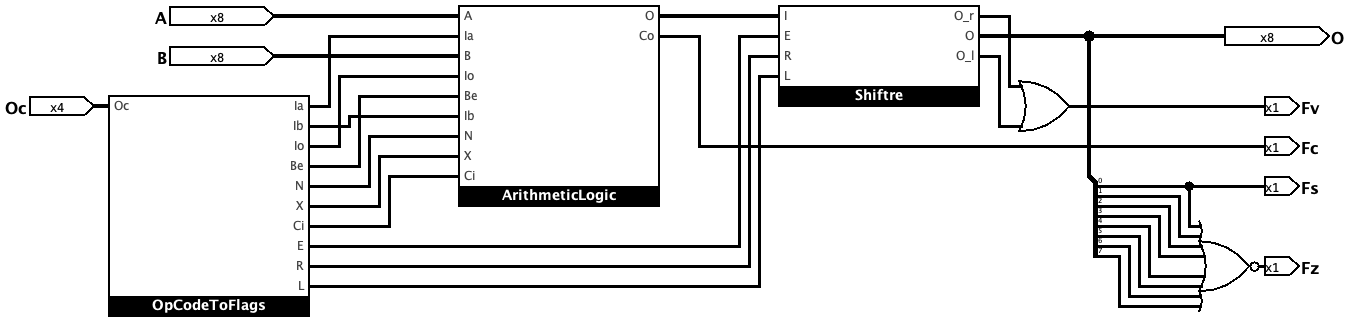
\includegraphics[scale=0.25]{ALU}
    \caption{ALU 회로도}
    \label{fig:alu}
\end{figure}

$O_c$ 값에 따라 수행되는 연산은 다음 \tablename{} \ref{tab:aluopc}과 같다.

\begin{table}
    \centering
    \begin{tabular}{rl|ll}
        $O_c$ & 연산 이름 & 연산 & 설명\\
        \hline
        \texttt 0 & A    & $A$ & A \\
        \texttt 1 & NOT  & $\neg A$ & NOT \\
        \texttt 2 & NEG  & $- A$ & NEGative \\
        \texttt 3 & SHL  & $A \ll 1$ & SHift Left \\
        \texttt 4 & INC  & $A + 1$ & INCrease \\
        \texttt 5 & DEC  & $A - 1$ & DECrease \\
        \texttt 6 & ADD  & $A + B$ & ADD \\
        \texttt 7 & SUB  & $A - B$ & SUBtract \\
        \texttt 8 & XOR  & $A \veebar B$ & eXclusive OR \\
        \texttt 9 & XNOR & $\neg (A \veebar B)$ & eXclusive Not OR \\
        \texttt A & AND  & $A \wedge B$ & AND \\
        \texttt B & NAND & $\neg (A \wedge B)$ & Not AND \\
        \texttt C & OR   & $A \vee B$ & OR \\
        \texttt D & NOR  & $\neg (A \vee B)$ & Not OR \\
        \texttt E & ASR  & $A \sim\gg 1$ & Arithmetic Shift Right \\
        \texttt F & LSR  & $A \gg 1$ & Logical Shift Right \\
    \end{tabular}
    \caption{ALU의 $O_c$ 값에 따라 계산되는 연산}
    \label{tab:aluopc}
\end{table}

\pagebreak

\subsection{Countre}

Countre는 매 클락마다 현재 수의 다음 수를 계산하는 부품이다.
Countre는 현재 실행하고 있는 명령어의 주소를 계산하는 데에 사용된다.

Countre는 $I$, $E_w$, $\textit{c}$의 입력 핀과
$O$, $c_o$의 출력 핀을 가지고 있다.
이중에서 $I$, $O$는 8비트 핀이다.
각각은 다음을 의미한다.

\begin{itemize}
    \item $I$ -- Input. $\overline{E_w}$일 때에 카운터에 적재할 값
    \item $E_w$ -- Enable $\overline{\textrm{Write}}$. 카운터를 실행한다.
        0으로 설정된 경우에는 $I$의 값을 카운터에 적재한다.
    \item $c$ -- Clock. 시스템 클락
    \item $O$ -- Output. 카운터에 적재되어있는 값
    \item $c_o$ -- Clock Overflowed. 카운터 확장을 위해 사용되는 클락.
        $\overline{O_7}$의 값과 같다.
\end{itemize}

\figurename{} \ref{fig:ctr}은 Countre의 회로도이고,
\tablename{} \ref{tab:ctr}은 Countre의 표이다.

\begin{figure}[h]
    \centering
    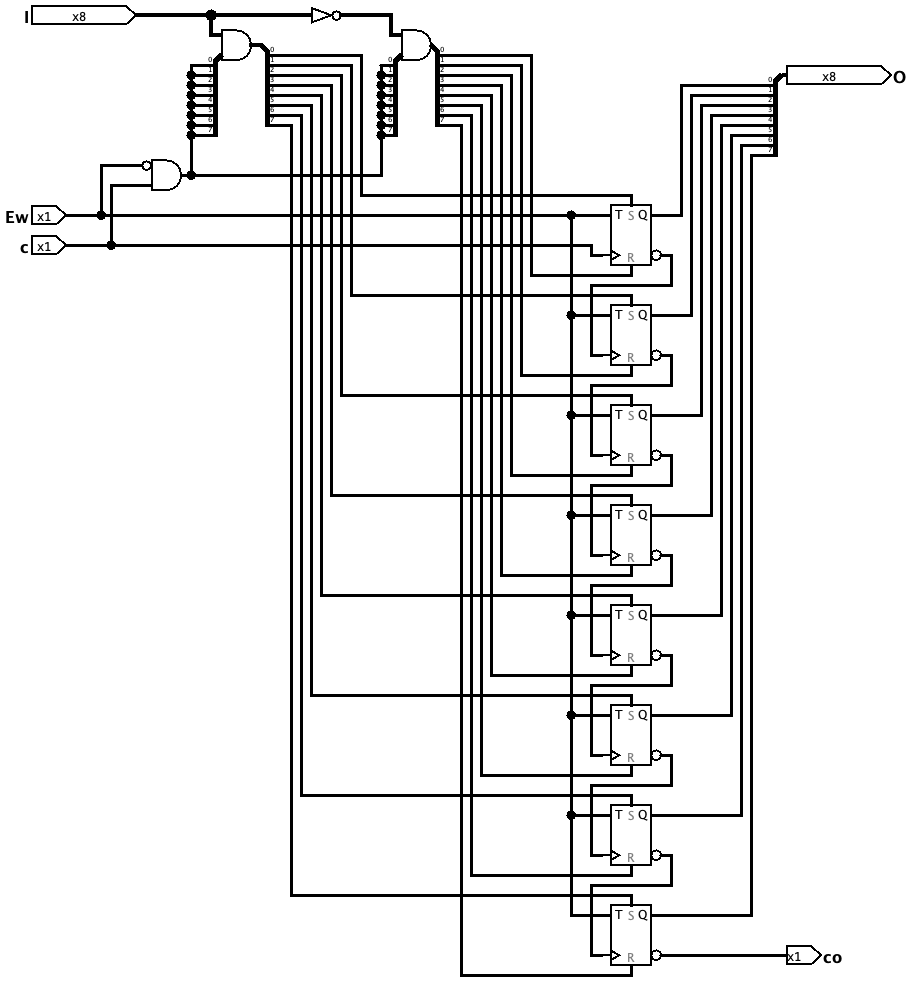
\includegraphics[scale=0.35]{Countre}
    \caption{Countre의 회로도}
    \label{fig:ctr}
\end{figure}

\begin{table}[h]
    \centering
    \begin{tabular}{cc|c}
        $I$ & $E_w$ & $O$ \\
        \hline
        $I$ & 0 & $O+1$ \\
        $I$ & 1 & $I$ \\
    \end{tabular}
    \caption{Countre의 표}
    \label{tab:ctr}
\end{table}

\section{CPU}

CPU는 Central Processing Unit의 약자로,
메모리에서 명령어를 읽어 해석하여 실행하는 부품이다.

CPU에는 메모리를 연결하여 프로그래밍할 수 있으며,
프로그래밍 방법에 대해서는 \ref{sec:machlang}장을 참고한다.

\subsection{제어 신호}

\begin{itemize}
    \item LO -- aLu Out
    \item AI -- A register In
    \item CI -- aCcumulator In
    \item OI -- Opcode register In
    \item PW -- Program counter Write
    \item PO -- Program counter Out
    \item DI -- aDdress register In
    \item MO -- Memory Out
    \item MI -- Memory In
    \item PE -- Program counter Enable
    \item II -- Instruction register In
\end{itemize}

\section{기계어}
\label{sec:machlang}

\end{document}
